\chapter{Value of Dynamic Schedule}

\section{Expected Cost Comparison}

Assume that there are $N$ customers to be scheduled. In the case of the static schedule, the expected cost of the optimal policy is given by $\phi (\mathbf{x}^{*}) = \phi (x_{1}^{*}, \ldots, x_{N - 1}^{*})$. In the case of the dynamic schedule, the expected cost of the optimal policy is given by $C_{N}^{*} (0)$.

Clearly, as the optimal policy for the dynamic schedule can match the optimal policy for the static schedule, $C_{N}^{*} (0) \leq \phi (\mathbf{x}^{*})$ regardless of the number of customers to be scheduled. Equality is attained for the cases where $N \in \{ 1, 2 \}$ as the schedules are identical in those cases.

\begin{figure}[htb]
	\centering
	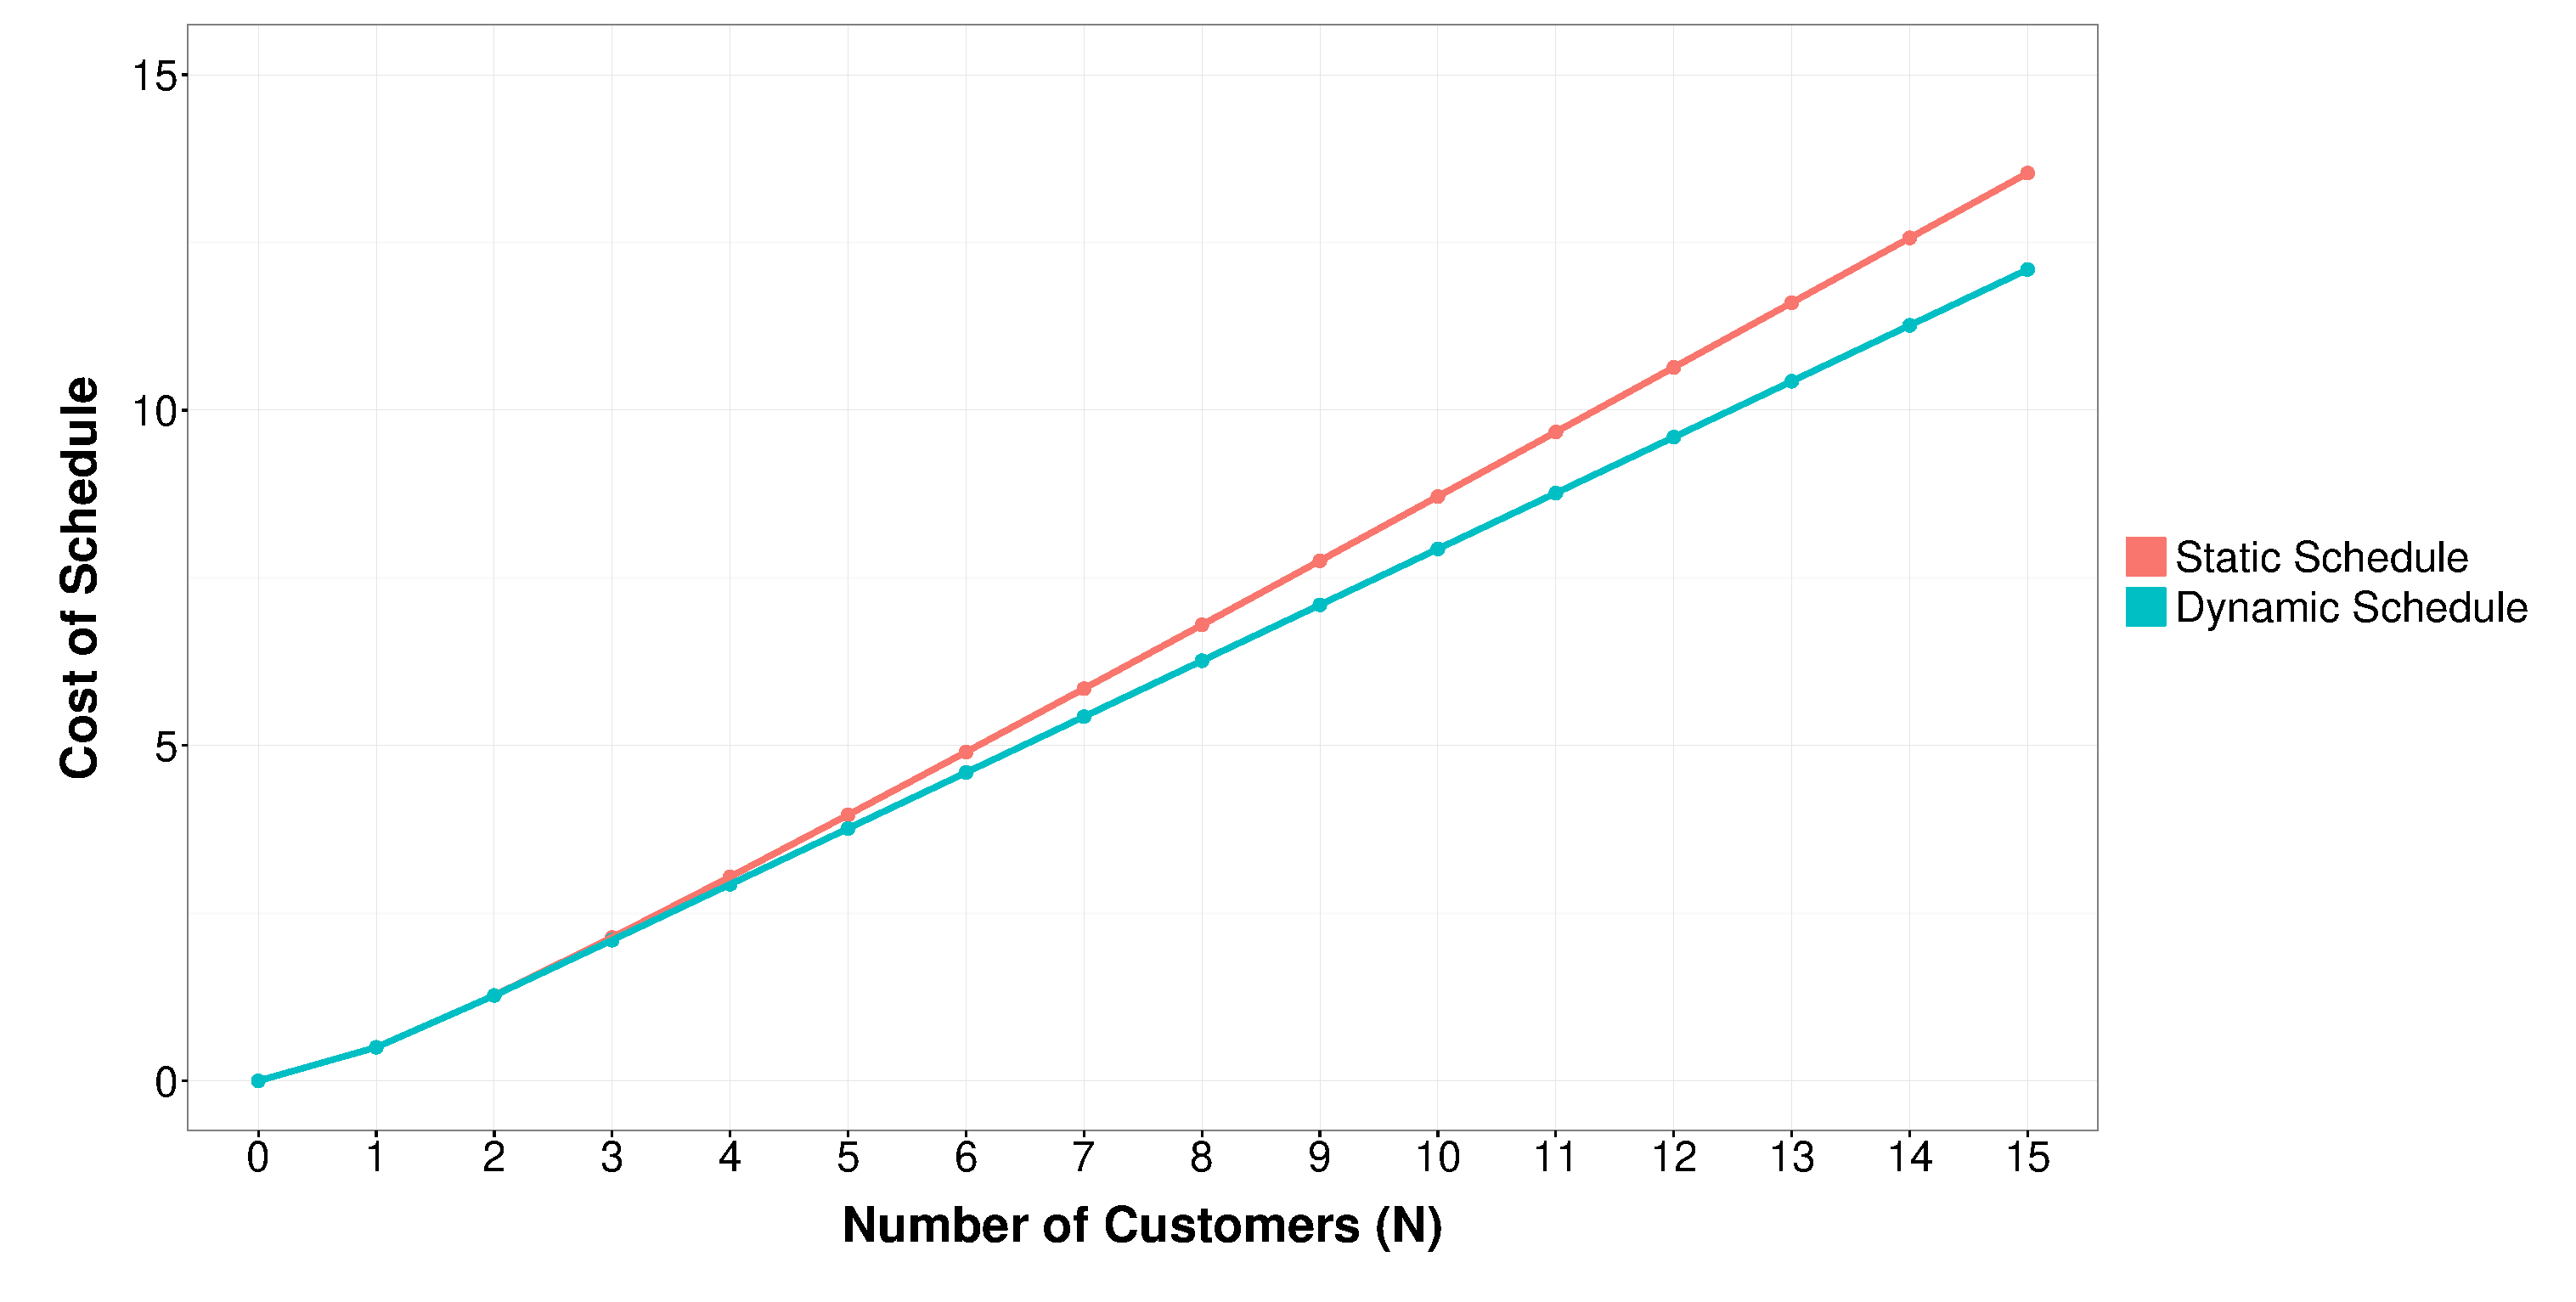
\includegraphics[width = 0.85\textwidth]{Comparison_Line_Cost_Num.eps}
	\caption{Plot of the expected cost of each schedule against the number of customers to be scheduled ($N$) for both the static and dynamic schedules where $N \in \{ 1, \ldots, 6 \}$, $\gamma = \frac{c_{S}}{c_{S} + c_{W}} = 0.5$ and $\mu = 1$.}
	\label{Graph_Cost_Comparison}
\end{figure}

Figure~\ref{Graph_Cost_Comparison} plots the expected costs of both the static and dynamic schedules against the number of customers to be scheduled ($N$) assuming $\gamma = 0.5$ and $\mu = 1$. As expected, the costs are identical for $N \in \{ 1, 2 \}$. For all other $N$ values, the cost of the static schedule is greater than the cost of the dynamic schedule. As $N$ increases, the difference between the costs increases.

\section{Percentage Cost Saving}

Define $\Delta C$  which measures the percentage difference between the cost of the static schedule and the dynamic schedule (i.e., the percentage cost saving).
\begin{equation}
	\Delta C = 100 \times \frac{\phi (\mathbf{x}^{*}) - C_{N}^{*} (0)}{\phi (\mathbf{x}^{*})}
\end{equation}

\begin{figure}[htb]
	\centering
	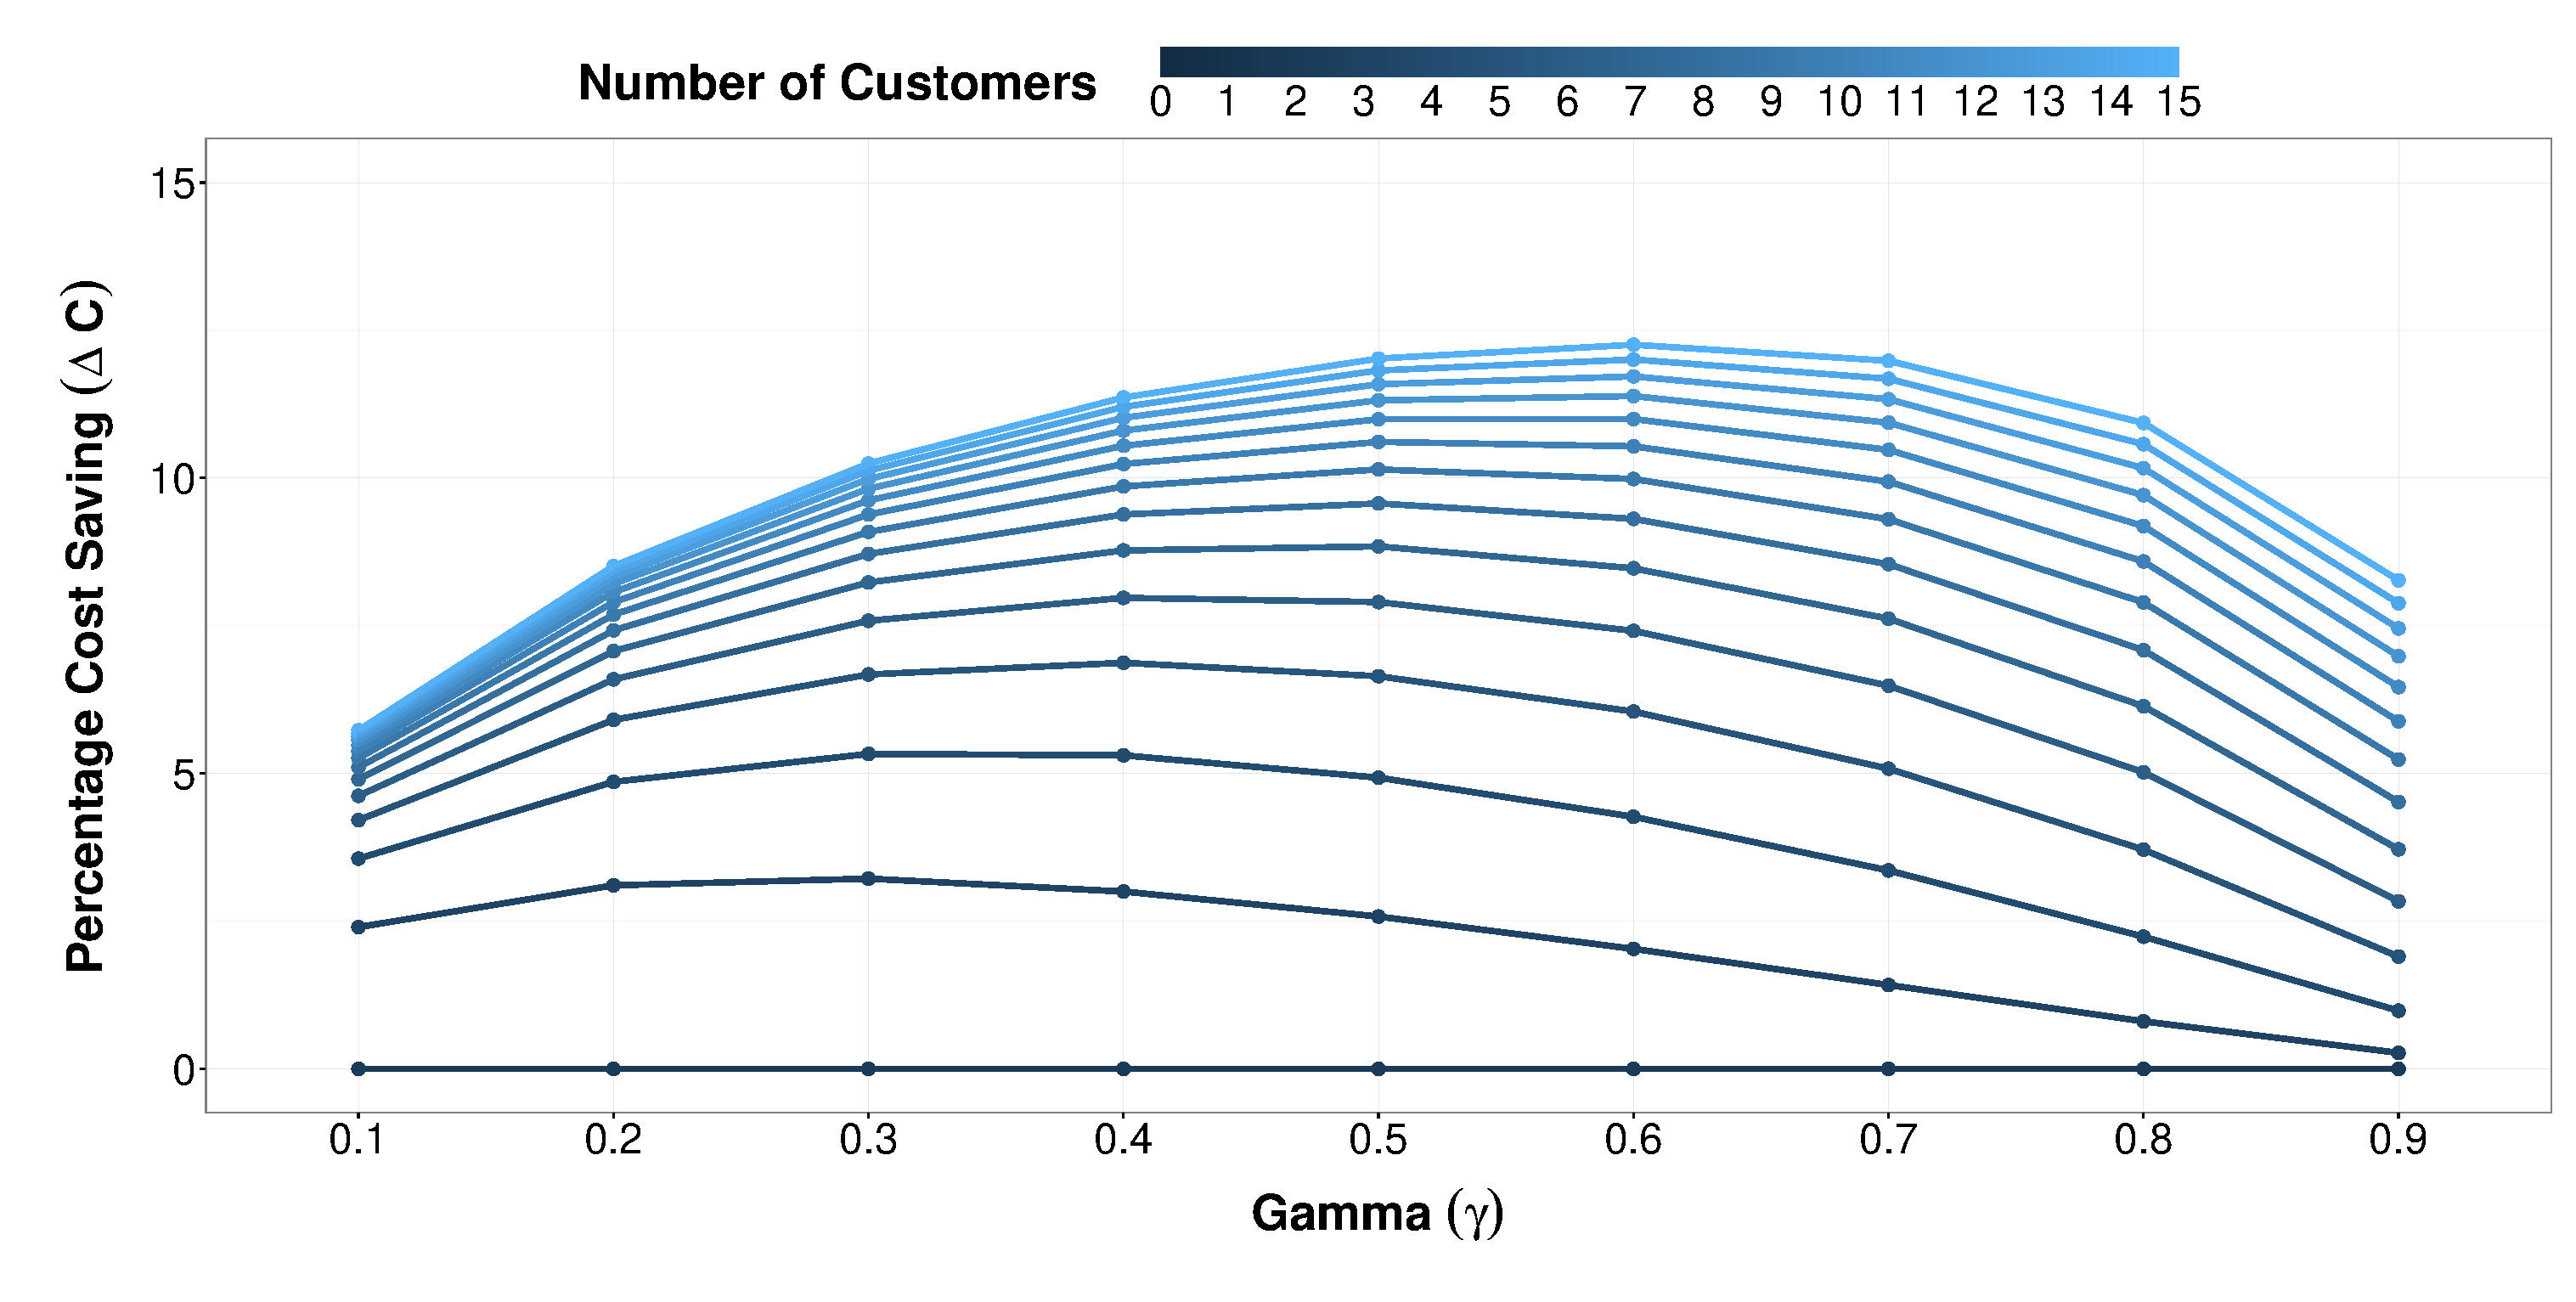
\includegraphics[width = 0.85\textwidth]{Cost_Saving_Line_Num.eps}
	\caption{Plot of the percentage cost saving ($\Delta C$) by using the dynamic schedule as opposed to the static schedule against $\gamma = \frac{c_{S}}{c_{S} + c_{W}}$ where $N = \{ 1, \ldots, 6 \}$ and $\mu = 1$.}
	\label{Graph_Cost_Saving}
\end{figure}

Figure~\ref{Graph_Cost_Saving} plots $\Delta C$ against $\gamma$ for various values of the number of customers to be scheduled ($N$). For $N \in \{ 1, 2 \}$, $\Delta C = 0$ for all values of $\gamma$ as the schedules are identical. As $N$ increases with $\gamma$ held constant, $\Delta C$ increases at a decreasing rate (i.e., the curves become closer together as $N$ increases).

For the maximum considered value of $\gamma$ (i.e., $\gamma = 0.95$), $\Delta C$ is at a minimum for all values of $N$. A large value of $\gamma$ indicates that the server availability cost per unit time is significantly greater than the waiting cost per unit time (i.e., $c_{S} \gg c_{W}$). As the server availability cost is heavily prioritised, there is little difference between the static and dynamic schedules, thus $\Delta C$ is small.

For each value of $N \geq 3$, the peak value of $\Delta C$ occurs at a middle value of $\gamma$. As $N$ increases, the peak occurs at a larger value of $\gamma$. For $N = 3, 4, 5$ and $6$, the peak occurs at $\gamma \approx 0.3, 0.35, 0.4$ and $0.45$ respectively.